% !TEX root = paper.tex
% !TEX encoding = UTF-8 Unicode

\section{Methodology}
\label{sec:methodology}



\begin{table*}[t]
\begin{subtable}[b]{.5\linewidth}
\begin{center}
\begin{tabular} { | c | p{66mm} | }
\hline
  12 & The post-edited translation is superior to the reference translation \\ \hline
  10 & The meaning of the Russian sentence is fully conveyed in the English translation \\ \hline
  8 & Most of the meaning of the Russian sentence is conveyed in the English translation \\ \hline
  6 & The English translation misunderstands the Russian sentence in a major way, or has many small mistakes \\ \hline
  4 & Very little information from the Russian sentence is conveyed in the English translation \\ \hline
  2 & The English translation makes no sense at all \\ \hline
\end{tabular}
\end{center}
\caption{Russian-English}
\label{judge_guidelines_russian}
\end{subtable}
\begin{subtable}[b]{.5\linewidth}
\begin{center}
\begin{tabular} { | c | p{66mm} | }
\hline
  10 & The meaning of the Spanish sentence is fully conveyed in the English translation \\ \hline
%  9 & The English translation contains one minor error \\ \hline
  8 & Most of the meaning of the Spanish sentence is conveyed in the English translation \\ \hline
  6 & The English translation misunderstands the Spanish sentence in a major way, or has many small mistakes \\ \hline
  4 & Very little information from the Spanish sentence is conveyed in the English translation \\ \hline
  2 & The English translation makes no sense at all \\ \hline
\end{tabular}
\end{center}
\caption{Spanish-English}
\label{judge_guidelines_spanish}
\end{subtable}
\caption{Adequacy evaluation guidelines for bilingual Russian-English human judges \citep{2014_WMT_Schwartz_etal}, and for bilingual Spanish-English human judges \citep{2009_EACL_Albrecht_etal}. Because no reference translation was available for Spanish-English, the 12 category is omitted.}
\label{judge_guidelines}
\end{table*}




\subsection{Russian-English Bilingual Participants}
There were six participants who served as post-editors in the Russian-English portion of this study, all of whom were paid for their time.
%
These participants were all English-Russian bilinguals.
%
Four of the six bilingual participants (PE2, PE3, PE4, \& PE6) had Russian as their first language (L1) and were highly proficient in English as their second language (L2).
%
The other two bilingual participants (PE1 \& PE5) had English as their first language and were highly proficient in Russian as their second language.
%
Three of the six bilingual participants were graduate students and three were undergraduate students; all were enrolled in a university Russian Translation program. %and three were undergraduate students in the same program.
%a Russian Translation program at the same American university.

%In addition, we made use of monolingual post-editing data previously released by \citet{2014_WMT_Schwartz_etal}.
%
%The relevant participant in that study was a native English speaker with no knowledge of Russian.

\subsubsection{Spanish-English Bilingual Participants}

There were four participants (PE7, PE8, PE9, PE10) who served as post-editors in this portion of the study, all of whom were paid for their time. 
%
They were all Spanish-English bilinguals with English as their first language (L1) and highly proficient in Spanish as their second language (L2). 
%
The four were second year students in a university Master of Spanish Translation program. 

\subsection{Russian Data}

We selected as source texts a subset of the texts from the 2014 Workshop on Statistical Machine Translation (WMT-14) shared translation task \citep{2014_WMT_Bojar_etal}.
%
Source texts were news articles covering world news events in late 2013.
%
The first text (Doc A) was originally a Russian-language BBC news article covering Syrian chemical weapons.
%
The second text (Doc B) was originally an English-language news article covering U.S. spying policy.
%
The texts were divided into segments that corresponded to sentences or stand-alone phrases (typically corresponding to news headlines, captions, or cutlines).
%
Segments in Doc A varied in length from 3 to 35 words (mean length 17 words); 
%
segments in Doc B varied in length from 9 to 55 words (mean length 23 words).


Professional translations of Doc A into English and Doc B into Russian were commissioned as part of the WMT-14 shared translation task \citep{2014_WMT_Bojar_etal}.
%
%Doc A consists of 27 segments; Doc B has 28 segments.
%
The Russian version of each text was translated automatically using Moses \citep{2007_ACL_Koehn} by \citet{2014_WMT_Schwartz_etal} as part of their WMT14 shared task submission.
%
As a side effect of the phrase-based MT process, Moses can be configured to produce alignment links, indicating which target language words were produced from which source language words.
%
To enable maximal comparability with the post-editing results of \citet{2014_WMT_Schwartz_etal}, we make use of those machine translations and alignments in this work.

% !TEX root = paper.tex
% !TEX encoding = UTF-8 Unicode


\begin{figure*}
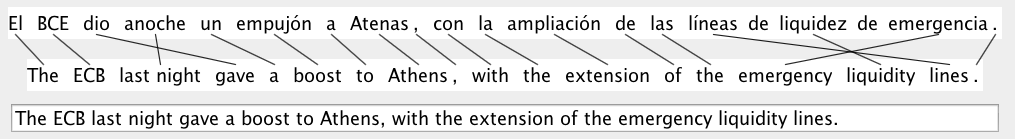
\includegraphics[width=\linewidth]{alignments_true}
\caption{Post-editing interface, with alignment links displayed. Sentence shown is from Spanish-English Doc C.}
\label{fig:screenshot_true}
\end{figure*}


\subsection{Spanish Data}

Two Spanish source texts were selected. Both were extracts from a news article from a Spanish newspaper covering current world news events. 
%
The two texts were divided up into segments that corresponded to sentences or stand alone phrases. 
%
The first text (Doc C) had 26 segments that varied in length from 4 to 24 words (mean length 15 words) and the second text (Doc D) had 25 segments that varied in length from 4 to 28 words (mean length 16 words).
%
No reference translations exist for either Spanish text.

The Spanish source texts were translated automatically using the Microsoft Bing Translator through its online developer API.
%
Bing Translator, when accessed via the developer API, can be configured to return character-level alignment links from source characters to target characters, in addition to  translated target language sentences.
%
Our scripts derive word alignments from the character alignments returned by the Bing Translator API.









\subsection{Russian-English Post-Editing Interface}

Each text was presented to post-editors in one of two variant modalities using the post-editing interface of \citet{2014_WMT_Schwartz_etal}. 
%
In both variants, each Russian source segment was presented along with the corresponding machine translated English segment; a text field (initially populated with the machine translated segment) where the post-editor could make changes was also presented.
%
In variant 1, the alignment links produced by Moses were graphically displayed, linking source words to their corresponding machine translated target words.
%
In variant 2, the alignment links were omitted from the visualization interface.


Each participant was instructed to edit one of the two texts using the interface where alignment links were shown,
%
and to edit the other text using the interface where alignment links were omitted.
%
Participants post-edited the two texts in one session lasting less than two hours, although there were no time limits set for the task.
%
Post-Editors 2, 4, and 6 were assigned to post-edit Doc A using the variant 1 interface that displayed alignments, and Doc B using the variant 2 interface that omitted alignments.
%
Post-Editors 1, 3, and 5 were assigned Doc A using variant 2 and Doc B using the variant 1 interface.

%For each of the segments there was also a reference translation created by XXXX.

\subsection{Spanish-English Post-Editing Interface}

Participants post-edited one text using the interface where alignment links were shown and the other text using the interface where alignment links were omitted. 
%
Participants post-edited the two texts in one session lasting less than one hour. 
%
Post-editors 7 and 9 edited Doc C using the interface that omitted the alignments and Doc D using the interface that displayed the alignments. 
%
Post-editors 8 and 10 edited Doc C using the interface that displayed the alignments and Doc D using the interface that omitted the alignments.

% !TEX root = paper.tex
% !TEX encoding = UTF-8 Unicode

\begin{figure}
\begin{subfigure}[b]{\linewidth}
\begin{center}
\caption{Russian-English}
\label{fig:mean_adequacy_score_ru}
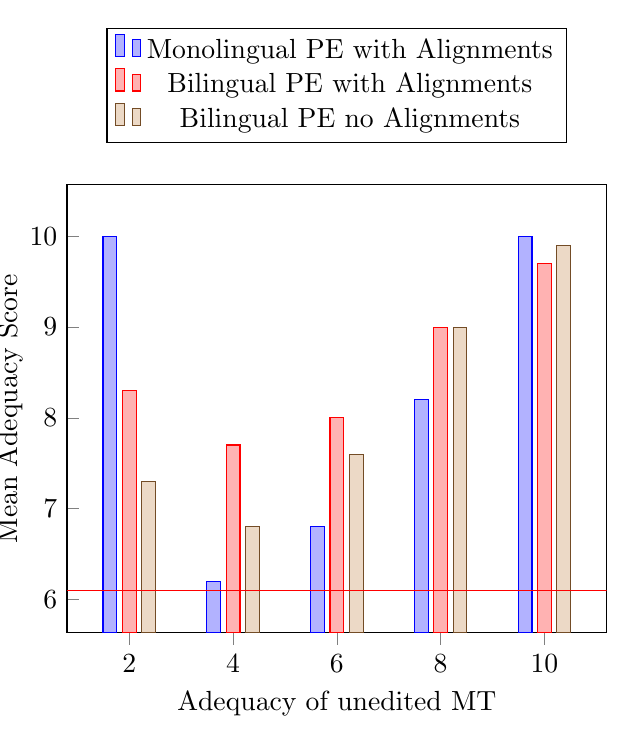
\begin{tikzpicture}[trim left={(-0.5,0)}]
\begin{axis}[
	%at={(10,0)},
	x tick label style={
		/pgf/number format/1000 sep=},
	ylabel shift={-0.15cm},
	ylabel=Mean Adequacy Score,
	enlargelimits=0.15,
	xtick pos=left,
	ytick pos=left,
	xlabel={Adequacy of unedited MT},
	%,
%	legend style={at={(0.5,-0.15)}},
%		anchor=north,legend columns=-1},
	legend style={at={(0.5,1.35)},anchor=north},
	ybar,
	bar width=5pt,
]
\addplot 
	coordinates {(2,10.0) (4,6.2)
		 (6,6.8) (8,8.2) (10,10)};

\addplot 
	coordinates {(2,8.3) (4,7.7)
		 (6,8.0) (8,9.0) (10,9.7)};

\addplot 
	coordinates {(2,7.3) (4,6.8)
		 (6,7.6) (8,9.0) (10,9.9)};

\addplot[red,sharp plot,update limits=false] 
	coordinates {(-1,6.1) (12,6.1)};

\legend{Monolingual PE with Alignments,Bilingual PE with Alignments,Bilingual PE no Alignments}
\end{axis}
\end{tikzpicture}
\end{center}
\end{subfigure}
\ \\
\begin{subfigure}[b]{\linewidth}
\begin{center}
\caption{Spanish-English}
\label{fig:mean_adequacy_score_es}
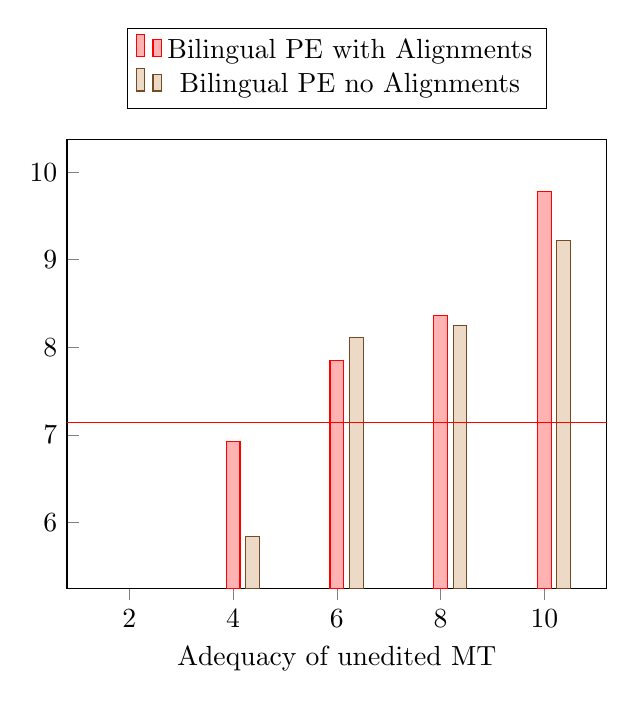
\begin{tikzpicture}[trim left={(-0.5,0)}]
\begin{axis}[
	%at={(10,0)},
	x tick label style={
		/pgf/number format/1000 sep=},
	ylabel shift={-0.15cm},
%	ylabel=Mean Adequacy Score,
	enlargelimits=0.15,
	xtick pos=left,
	ytick pos=left,
	xlabel={Adequacy of unedited MT},
	legend style={at={(0.5,1.25)},anchor=north},
	ybar,
	xmin=2,
	bar width=5pt,
]
\addplot 
	coordinates {};

%	Adequacy with align	Adequacy w/o align
%2		
%4	6.92	5.84
%6	7.85	8.11
%8	8.36	8.25
%10	9.78	9.22

\addplot coordinates {(4,6.92) (6,7.85) (8,8.36) (10,9.78) };
\addplot coordinates {(4,5.84) (6,8.11) (8,8.25) (10,9.22) };
\addplot[red,sharp plot,update limits=false] coordinates { (-1,7.14) (12,7.14) };
	
%\addplot coordinates {(4,6.6) (6,7.7272727272727275) (8,8.818181818181818) (10,9.923076923076923) };
%\addplot coordinates {(4,6.0) (6,8.090909090909092) (8,8.909090909090908) (10,9.384615384615385) };
%\addplot[red,sharp plot,update limits=false] coordinates { (-1,7.686274509803922) (12,7.686274509803922) };

\legend{Bilingual PE with Alignments,Bilingual PE no Alignments}
\end{axis}
\end{tikzpicture}
\end{center}
\end{subfigure}
\caption{Mean adequacy score, categorized by the adequacy score of the unedited MT. The red horizontal line indicates the mean adequacy score (Russian-English: 6.1; Spanish-English: 7.1) of the unedited MT.}
\label{fig:mean_adequacy_score}
\end{figure}



\subsection{Procedure}

Participants performed the test individually in an office setting and were instructed to minimally post-edit. 
%
Specifically, participants were asked to disregard issues of style and to focus on 
%
a) how well the translation conveyed the meaning of the source text, and 
%
b) the grammatical correctness of the translated segments. 
%
Participants sat in front of a computer that displayed the source texts divided up into segments (see Figure \ref{fig:screenshot_true} \vpageref[above]{fig:screenshot_true}). % (see \citet{2014_WMT_Schwartz_etal}).
%
Directly below each source text segment, its machine translation was displayed.
%
Below that was an active response area, where participants were asked to carry out the post-editing.

During initial data collection (the Russian-English condition), the only data collected was the final post-edited output and the overall time taken per text.
%
Subsequently, we enhanced the post-editing software with additional logging functionality, enabling the software to record key-logging and mouse-logging data.
%
For the subsequent Spanish-English condition, this enhanced software was utilized; for this condition millisecond-precision keyboard-event and mouse-event logs were recorded in addition to collecting final post-edited output and overall time taken per text.

We believe that scientific inquiry is at its strongest when experiments can be easily replicated, and when the raw and processed data from such experiments can be directly verified by reviewers, readers, and other experimenters.
%
In that spirit, all data and code produced or used in this work are provided in the attached dataset and software supplements.
%
This includes all logs, along with raw machine translation output, alignment data, post-edited output, adequacy judgements, post-editing software, and supplementary scripts.



